\section{Основные понятия теории вероятностей}
\subsection{Предмет статистической радиофизики}

Статистическая радиофизика изучает случайные явления в радиофизике.
Статистическое описание является наиболее подходящим для многих электромагнитных
явлений. Статистическая радиофизика изучает случайные процессы на всех этапах
радиосвязи.

Статистическая радиофизика использует методы радиофизики, статистической физики
и теории вероятностей и работает с информационными характеристиками (дисперсией,
корреляцией, \ldots).

Под сообщением понимаются любые данные или сведения, подлежащие передаче. По
своей природе сообщения делятся на механические, тепловые, электромагнитные и
т.д. Сообщения неэлектрической природы часто преобразуют в электрический сигнал
при помощи преобразователей. При необходимости, электрический сигнал для
передачи преобразуют в радиосигнал.

При преобразовании, передаче, распространении и приёме сигнал подвергается
искажениям. Они обуславливаются:
\begin{enumerate}
    \item внешними и внутренними помехами;
    \item распространением сигнала через турбулентную среду;
    \item техническим несовершенством устройств.
\end{enumerate}
Любые нежелательные возмущения, накладывающиеся на сигнал, называются шумом.

\subsection{Вероятность}

Основное понятие радиофизики -- случайная величина. Случайная величина -- это
форма представления заранее не предсказуемых результатов опыта. Для описания
случайных величин в математике вводится понятие вероятности.

Вероятность события \( A \) есть отношение числа опытов, в которых происходило
это событие, к общему числу опытов при стремлении числа опытов к бесконечности:
\[
    P(A) = \lim_{N\to\infty}\frac{N_A}{N}.
\]

Если событие не может произойти ни в одном опыте, то вероятность такого события
равна нулю, а событие называется невозможным.

Если же событие происходит в каждом опыте, то его вероятность равна единице, а
само событие называется достоверным.

Если два события никогда не происходят вместе, то такие события называются
несовместимыми.

Событие, представляющее собой множество вероятных исходов составляет группу
событий. Группа называется полной, если в результате опыта произойдёт одно из
событий этой группы.

Два события, образующие полную группу, называются противоположными, если они
несовместимы.

Если всякий раз, когда происходит событие \( A \), происходит событие \( B \),
то говорят, что \( A \) влечёт за собой \( B \): \( A \subset B \). Если
\( A \subset B \) и \( B \subset A \), то \( A = B \) и такие события называют
равносильными или эквивалентными.

Событие \( A \) называется статистически зависимым от события \( B \), если
\( P(A) \) зависит от того, осуществилось ли событие \( B \) или нет. В случае
статистической зависимости можно ввести условную вероятность \( P(A|B) \)
события \( A \) при осуществлении события \( B \). Безусловные вероятности
называются априорными, а условные -- апостериорными.

Произведением событий называется такое событие, которое происходит, когда
одновременно происходят все эти события:
\[
    P(AB) = P(A) \cdot P(B|A) = P(B) \cdot P(A|B).
\]

Суммой событий называется событие, которое происходит тогда и только тогда,
когда происходит хотя бы одно из этих событий:
\[
    P(A+B) = P(A) + P(B) - P(AB).
\]

Если события несовместимы и образуют полную группу, то
\[
    P\left(\sum A_i\right) = \sum P(A_i) = 1.
\]
Это условие называется условием нормировки.

Пусть несовместимые события \( B \) и \( C \) входят в полную группу, а \( A \)
может произойти только при наступлении этих двух событий, тогда
\[
    P(A) = P(AB) + P(AC) = P(B) \cdot P(A|B) + P(C) \cdot P(A|C).
\]
Эта формула называется формулой полной вероятности.
\[
    P(B|A) = \frac{P(AB)}{P(A)} = \frac{P(B) \cdot P(A|B)}
    {P(B) \cdot P(A|B) + P(C) \cdot P(A|C)} \text{ -- формула Байеса.}
\]

В технике используются системы, состоящие из нескольких элементов. Надёжностью
системы называют вероятность того, что система будет работать без отказа в
течение установленного промежутка времени. Пусть система состоит из двух
элементов, причём надёжность первого \( P_1 \), а второго \( P_2 \). Тогда
надёжность при последовательном соединении равна \( P_1P_2 \),  а при
параллельном~--\\ \( 1 - (1 - P_1)(1 - P_2) = P_1 + P_2 - P_1P_2 \).

\subsection{Функция распределения случайной величины}

Соотношение, устанавливающее связь между возможным значением случайной величины
и её вероятностью, называется функцией распределения.

Пусть случайная величина \( X \) каким-либо образом распределена на
\( \mathbb{R} \). Тогда \( F(x) = P(X \le x) \) называется (интегральной)
функцией распределения величины \( X \). Эта функция обладает следующими
свойствами:
\begin{itemize}
    \item для дискретной величины \( \ds F(x) = \sum_{X_i \le x}P(X_i) \);
    \item для непрерывной величины \( \ds F(x) = \int_{-\infty}^x w(\xi)d\xi \);
    \item \( F(-\infty) = 0 \);
    \item \( F(+\infty) = 1 \);
    \item \( F(x) \) -- монотонно неубывающая функция;
    \item \( P(x_1 < X < x_2) = F(x_2) - F(x_1) \);
    \item для непрерывно распределённой величины является гладкой всюду
        непрерывной функцией.
\end{itemize}
В случае непрерывной величины функция
\[
    w(x) = \der{F(x)}{x}
\]
называется плотностью распределения. Она обладает рядом свойств:
\begin{itemize}
    \item \( \ds \int_{-\infty}^{+\infty} w(\xi) d\xi = 1 \);
    \item \( \forall x\ w(x) \ge 0 \);
    \item для дискретной величины
        \( \ds w(x) = \sum_i P(X_i) \cdot \delta(x - X_i) \).
\end{itemize}

Для любой функции случайной величины можно ввести понятие среднего значения
\[
    \average{f(x)} = \int_{-\infty}^{+\infty}f(x)w(x)dx,
\]
переходящее для дискретной величины в
\[
    \average{f(x)} = \sum_i P(X_i)f(X_i).
\]

\subsection{Моменты случайной величины}

Момент \( m_n \) \( n \)-го порядка определяется выражением
\[
    m_n(X) = \average{X^n} = \int_{-\infty}^{+\infty} x^n w(x) dx.
\]
\( m_1 \) называется средним значением или математическим ожиданием.

Центральный момент \( \mu_n \) \( n \)-го порядка определяется выражением
\[
    \mu_n(X) = \average{\left(X - \average{X}\right)^n}.
\]
\( \mu_2 = \sigma^2 \) называется дисперсией, а \( \sigma \) --
среднеквадратичным отклонением.

\subsection{Неравенство Чебышёва}
    Рассмотрим определение дисперсии
    \[
        \sigma^2 = \int_{-\infty}^{+\infty} (x - \average{x})^2w(x)dx.
    \]
    Разобьём этот интеграл на три:
    \[
        \sigma^2 = \int_{-\infty}^{\average{x}-n\sigma}(x-\average{x})^2w(x)dx +
        \int_{\average{x}-n\sigma}^{\average{x}+n\sigma}(x-\average{x})^2w(x)dx+
        \int_{\average{x}+n\sigma}^{+\infty}(x-\average{x})^2w(x)dx.
    \]
    Второй интеграл в сумме -- это вероятность того, что
    \( X \in [\average{x} - n\sigma, \average{x} + n\sigma] \). По смыслу он
    больше нуля, поэтому имеет место неравенство:
    \[
        \sigma^2 \ge \int_{-\infty}^{\average{x}-n\sigma}(x-\average{x})^2w(x)dx +
        \int_{\average{x}+n\sigma}^{+\infty}(x-\average{x})^2w(x)dx.
    \]
    В этих областях интегрирования \( \abs{x-\average{x}} \ge n\sigma \),
    поэтому
    \[
        \sigma^2 \ge n^2\sigma^2 \left[
            \int_{-\infty}^{\average{x}-n\sigma}w(x)dx +
            \int_{\average{x}+n\sigma}^{+\infty}w(x)dx
        \right] = n^2\sigma^2P(\abs{x-\average{x}} \ge n\sigma),
    \]
    \[
        P(\abs{x-\average{x}} \ge n\sigma) \le \frac{1}{n^2}.
    \]
    Последнее неравенство называется неравенством Чебышёва. Оно показывает, что
    вероятность того, что флуктуация будет больше \( n\sigma \) стремительно
    падает с ростом \( n \).
\subsection{Совместное распределение}
Для двух случайных величин \( X \) и \( Y \) можно ввести двухмерную функцию
распределения \( F(x,y) = P(X \le x, Y \le y) \). Эта функция обладает всеми
свойствами одномерной функции распределения. Кроме того,
\( F(x, +\infty) = F_x(x) \). Для непрерывно распределённых величин можно ввести
плотность распределения
\[
    w(x,y) = \pcder{F(x,y)}{x}{y} \ge 0.
\]
Тогда
\[
    F(x, y) = \int_{-\infty}^x\int_{-\infty}^y w(\xi,\eta)d\xi d\eta,\quad
    F_x(x) = \int_{-\infty}^x\int_{-\infty}^{+\infty} w(\xi,\eta)d\xi d\eta.
\]

Для независимых событий
\( F(x,y) = F_x(x) \cdot F_y(y), w(x,y) = w_x(x) \cdot w_y(y) \).

Для зависимых можно ввести условную функцию распределения
\begin{gather*}
    F(y|x) = \lim_{\xi \to x} P(\xi < X \le x, Y \le y),\quad
    w(y|x) = \pder{F(y|x)}{y} \ge 0,\\
    w_y(y) = \int_{-\infty}^{+\infty} w(y|x) w_x(x) dx.
\end{gather*}

Смешанный момент
\[
    m_{kn} = \int_{-\infty}^{+\infty}\int_{-\infty}^{+\infty}x^ky^nw(x,y)dxdy,
\]
центральный момент
\[
    \mu_{kn} = \int_{-\infty}^{+\infty}\int_{-\infty}^{+\infty}
        \left(x-\average{X}\right)^k
        \left(y-\average{Y}\right)^n w(x,y)dxdy.
\]
Очевидно, что
\[
    \average{X} = m_{10},\ \average{Y} = m_{01},\ \sigma_x^2 = \mu_{20},
    \ \sigma_y^2 = \mu_{02}.
\]
\( B = m_{11} \) называется ковариацией, а
\[
    r = \frac{B}{\sigma_x\sigma_y}
\]
корреляционным моментом. Для независимых случайных величин оба этих числа равны
нулю. В этом случае случайные величины называются ортогональными.

\subsection{Задачи}
\begin{enumerate}
    \item По линии связи в случайном порядке передаются 30 знаков русского
        алфавита. Найти вероятность того, что на ленте появится
        последовательность букв, образующая слово ``радио'' при передачи 5
        знаков.

        5 букв из 30 с учётом их порядка можно выбрать
        \( A_{30}^{5} = 30\cdot29\cdot28\cdot27\cdot26 \) способами.
        Следовательно, вероятность того, что эти 5 букв составят слово ``радио''
        равна
        \[
            \frac{1}{30\cdot29\cdot28\cdot27\cdot26} = 5.8\cdot10^{-8}.
        \]
    \item В партии из 10 радиоламп имеются 4 нестандартные. Для проверки
        выбирают наугад 5 радиоламп. Определите вероятность того, что среди них
        будут 2 нестандартные.

        5 ламп из 10 можно выбрать \( C_{10}^5 \) способами. При этом, среди них
        должно оказаться 2 нестандартные, которые можно выбрать \( C_4^2 \)
        способами, и 3 стандартные, которые выбираются \( C_6^3 \) способами.
        Искомая вероятность определяется формулой
        \[
            \frac{C_6^3 \cdot C_4^2}{C_{10}^5} = \frac{10}{21}.
        \]
    \item В любой момент интервала времени \( T \) равновозможно поступление
        двух независимых сигналов. Приёмник будет перегружен, если разность
        между моментами поступления сигнала будет меньше \( \tau \). Определить
        вероятность перегруза.
        \begin{figure}[h]
        \begin{center}
            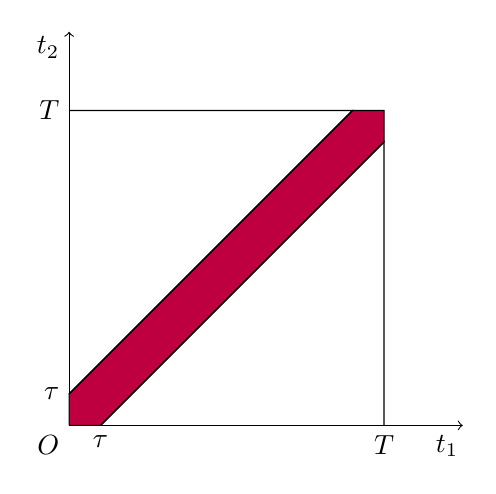
\begin{tikzpicture}
                \draw [<->] (0, 5) -- (0, 0) -- (5, 0);
                \node [below] at (4.8, 0) {\( t_1 \)};
                \node [left] at (0, 4.8) {\( t_2 \)};
                \draw [fill=purple] (0, 0) -- (0.4, 0) -- (4, 3.6) -- (4, 4) --
                    (3.6, 4) -- (0, 0.4) -- (0, 0);
                \draw (0.4, 0) -- (4, 3.6) -- (4, 0);
                \draw (0, 0.4) -- (3.6, 4) -- (0, 4);
                \node [below] at (0.4, 0) {\( \tau \)};
                \node [below] at (4, 0) {\( T \)};
                \node [below left] at (0, 0) {\( O \)};
                \node [left] at (0, 0.4) {\( \tau \)};
                \node [left] at (0, 4) {\( T \)};
            \end{tikzpicture}
        \end{center}
        \end{figure}

        Воспользуемся геометрической вероятностью. Для этого изобразим все
        возможные времена приёма сигналов на плоскости. Тогда все возможные
        события образуют квадрат со стороной \( T \). Область, соответствующая
        перегрузке определяется условием \( |t_1 - t_2| \le \tau \) и
        представляет из себя закрашенный шестиугольник. Тогда вероятность
        перегрузки определяется выражением
        \[
            \frac{T^2 - (T-\tau)^2}{T^2} =
            \frac{\tau}{T}\left(2 - \frac{\tau}{T}\right).
        \]

    \item Два стрелка стреляют по очереди до первого попадания. Каждый из них
        имеет право сделать не более двух выстрелов. Вероятности попадания в
        мишень при одиночном выстреле равны \( P_1 \) и \( P_2 \)
        соответственно. Найти вероятности попадания в мишень для каждого из
        стрелков.

        Первый стрелок может поразить мишень либо первым выстрелом, либо после
        своего промаха и промаха второго:
        \[
            P_I = P_1 + (1 - P_1)(1 - P_2)P_1.
        \]
        Второй может поразить мишень либо после промаха первого, либо после
        промаха первого, своего и ещё одного промаха первого:
        \[
            P_{II} = (1 - P_1) P_2 + (1 - P_1)(1 - P_2)(1 - P_1)P_2.
        \]
    \item Определить надёжность схемы, представленной на рисунке.
        \begin{figure}[h]
        \begin{center}
        \begin{circuitikz}
            \draw (0, 0) to [short,o-] (1,0);
            \draw (1, 0) to [short] (1,2);
            \draw (1, 0) to [short] (1,-2);
            \draw (1, 2) to [generic, l^=\( P_1 \)] (3,2);
            \draw (3, 2) to [generic, l^=\( P_2 \)] (5,2);
            \draw (1, 0) to [generic, l^=\( P_3 \)] (5,0);
            \draw (1, -2) to [generic, l^=\( P_4 \)] (5,-2);
            \draw (5, 2) to [short] (5,0);
            \draw (5, -2) to [short] (5,0);
            \draw (5, 0) to [short,-o] (6,0);
        \end{circuitikz}
        \end{center}
        \end{figure}

        Для параллельного соединения надёжность определяется выражением
        \[
            P = 1 - (1 - P_{12})(1 - P_3)(1 - P_4),
        \]
        где \( P_{12} = P_1 \cdot P_2 \) -- надёжность последовательного
        соединения в верхней ветке.

    \item По каналу связи, подверженному воздействию помех, передаётся одна из
        команд управления в виде кодовых комбинаций \( 00000 \) и \( 11111 \),
        причём априорные вероятности передачи этих команд равны \( 0,3 \) и
        \( 0,7 \) соответственно. Из-за наличия помех вероятность приёма символа
        правильно уменьшается до \( 0,6 \). На выходе приёмника зарегистрирована
        комбинация \( 10110 \). Определить, какая команда была передана.

        Обозначим передачу последовательности \( 00000 \) как событие \( 0 \),
        передачу последовательности \( 11111 \) как событие \( 1 \), а приём
        последовательности \( 10110 \) как событие \( A \). Требуется
        определить, какая последовательность была передана, то есть требуется
        определить условные вероятности \( P(1|A) \) и \( P(0|A) \). По формуле
        Байеса
        \[
            P(1|A) = \frac{P(A1)}{P(A)},\ P(0|A) = \frac{P(A0)}{P(A)} =
            1 - P(1|A).
        \]
        \[
            P(A) = P(A1) + P(A0),
        \]
        \[
            P(A1) = P(1) \cdot P(A|1) = 0,7\cdot(0,6)^3\cdot(0,4)^2,
        \]
        \[
            P(A0) = P(0) \cdot P(A|0) = 0,3\cdot(0,6)^2\cdot(0,4)^3.
        \]
        Подставив числа в первую формулу, получим
        \[
            P(1|A) = 0,78,\ P(0|A) = 0,22.
        \]
        Следовательно, была передана последовательность \( 11111 \).

    \item Противотанковое орудие ведёт стрельбу по танку. Всего производится 6
        выстрелов. Вероятность попасть в танк при выстреле равна \( 0,3 \).
        Определить наивероятнейшее число попаданий в танк и число выстрелов,
        необходимое, чтобы с вероятностью \( 0,9 \) поразить танк.

        Число попаданий в танк является случайной величиной, подчиняющейся
        биномиальному распределению. Наивероятнейшее значение в случае
        биномиального распределения определяется неравенством
        \[
            (n+1)p - 1 \le m \le (n+1)p.
        \]
        Подставляя числа, получаем
        \[
            7\cdot0.3 - 1 \le m \le 7\cdot0,3 \Rightarrow m = 2.
        \]
        Вероятность не попасть в танк после \( n \) выстрелов равна
        \( (1 - 0,3)^n = 0,7^n \). Следовательно, вероятность попасть
        \( 1 - 0,7^n \), а из условия \( 1 - 0,7^n \ge 0,9 \) получаем
        \( n = 7 \).

    \item Посадочная система аэропорта обеспечивает заход на посадку самолётов с
        интервалом не менее 5 минут. Два самолёта должны прибыть по расписанию с
        разностью 10 минут. Какова вероятность того, что второму самолёту
        придётся уйти в зону ожидания, если первый самолёт может выйти на
        аэродром с отклонением в 10 минут от расписания, а второй -- в пределах
        5 минут.

        \begin{figure}[h]
        \begin{center}
            \begin{tikzpicture}[x=11, y=8.5]
                \draw [->] (-11, 0) -- (11, 0);
                \draw [->] (0, -1) -- (0, 16);
                \node [below] at (11.2, 0) {\( t_1 \)};
                \node [left] at (0, 15.8) {\( t_2 \)};
                \draw [thick] (-10, -.1) node [below] {\( -10 \)} -- (-10, .1);
                \draw [thick] (10, -.1) node [below] {\( 10 \)} -- (10, .1);
                \draw [thick] (-.1, 5) node [right] {\( 5 \)} -- (.1, 5);
                \draw [thick] (-.1, 15) node [right] {\( 15 \)} -- (.1, 15);
                \draw [dashed] (-10, 5) -- (10, 5) -- (10, 15) -- (-10, 15) --
                    (-10, 5);
                \draw (0, 5) -- (10, 15);
                \node [left] at (7, 13) {\( t_2 = t_1 + 5 \)};
                \node at (-4, 7)
                    {\parbox{4.5cm}{второй сможет сесть по прибытии}};
                \node at (7, 7)
                    {\parbox{2.5cm}{второй ожидает}};
            \end{tikzpicture}
        \end{center}
        \end{figure}

        Рассматриваемое множество событий можно отобразить на прямоугольник со
        штриховой границей, представленный на рисунке. Условие интервала между
        посадками приводит к тому, что события под прямой \( t_2 - t_1 = 5 \)
        соответствуют случаю, в котором второй самолёт уходит в зону ожидания.
        Нетрудно видеть, что площадь треугольника составляет четверть
        от площади прямоугольника, поэтому и вероятность равна \( P = 0,25 \).
\end{enumerate}
